\documentclass[aspectratio=169,11pt]{beamer}
\usetheme{default}\usecolortheme{seagull}
\usepackage{booktabs,tabularx,amsmath,hyperref}
\setbeamertemplate{navigation symbols}{}
\setbeamertemplate{footline}{\hfill\scriptsize\insertframenumber/\inserttotalframenumber\hspace{2em}\vspace{1em}}
\setbeamertemplate{itemize items}{--}
\setbeamerfont{frametitle}{size=\large,series=\bfseries}
\setbeamercolor{frametitle}{fg=black}\setbeamercolor{title}{fg=black}
\definecolor{expred}{HTML}{B0413E}\definecolor{bureaublue}{HTML}{2C5F8A}
\newcommand{\m}[1]{\item #1}
\newcommand{\backup}[2]{\hfill{\scriptsize\hyperlink{#1}{\textcolor{bureaublue}{$\rightarrow$ #2}}}}
\newcommand{\backto}{\hfill{\scriptsize\hyperlink{main-end}{\textcolor{bureaublue}{$\leftarrow$ main}}}}
\title{Revealed Preference Discount Rates}
\subtitle{Can default choices reveal time preferences?}
\author{Joseph Hall\\Georgia Tech}
\date{September 2026}
\begin{document}
\begin{frame}[plain]\titlepage\end{frame}

\begin{frame}{What the paper does}
\begin{itemize}
\m{A borrower who defaults trades the payment due now against penalties that arrive later. The theory shows that the responses of default to payments due at different dates identify the discount function, with no consumption data and no utility function beyond concavity.}
\m{Applied within borrower to a credit-bureau panel of auto loans, the formula gives an annual discount rate of $0.11$ over the horizon of a contract, with a 95 percent set from $0.09$ to $0.13$.}
\m{The rate varies non-monotonically with credit score and income. It is steepest near median credit scores and at the lowest incomes, and nowhere rises with the group's default rate, which falls fifty-fold across the same score deciles.}
\m{The one gradient is age. Borrowers aged 18 to 30 reveal $0.32$, and every older group reveals zero.}
\end{itemize}
\end{frame}

\begin{frame}{The identity}
Response of default to a payment due $s$ months ahead $=$ common scale $\times$ date-specific weight
\[ \frac{\partial p}{\partial m_s} \;=\; \phi \cdot D(s-1)\, Q_s\, \lambda_s \qquad (\text{discount function} \times \text{survival} \times \text{marginal-utility ratio}) \]
\begin{itemize}
\m{Two payment paths in one population. The ratio of responses cancels $\phi$ and, with survival measured, identifies $D$.}
\m{In logs the weight is the Euler equation's decomposition of the rate a household demands to defer a dollar, $-\log w_s = \rho(s-1)/12 - \log\lambda_s - \log Q_s$. Impatience is $\rho$. Consumption smoothing is $\lambda_s$, and it is measured.}
\m{The identity replaces marginal willingness to save, the variation asset prices use, with marginal willingness to avoid default. It measures the time preferences of households with debt and no assets.}
\end{itemize}
\backup{bk-theory}{propositions}
\end{frame}

\begin{frame}{Two provisos, two results}
\begin{enumerate}
\item \textbf{The present-payment premium.} The payment due now is valued at the marginal defaulter's marginal utility and later ones at a repayer's, so $\lambda_s < 1$. Present bias $\beta$ and $\lambda_s$ enter every response as the product $\beta\lambda_s$, and no experiment that moves payments across dates separates them (Theorem). A liquid dollar against an illiquid dollar at one date does, and Indarte's pair measures the level at $0.2$.
\item \textbf{Beliefs.} Subjective survival multiplies $D$. The discount function is identified with beliefs fixed, and the panel fixes them at measured survival.
\end{enumerate}
\backup{bk-limits}{the theorems}
\end{frame}

\begin{frame}{A default within a window is a decision at its own month}
\[ R_K \;=\; \frac{\sum_{t \le K}\omega_t\, T\, w_{T-t+1}}{\sum_{t \le K}\omega_t \sum_{k \le T-t+1} w_k}, \qquad w_1 = 1, \quad w_k = \lambda_k\,e^{-(\rho + h)(k-1)/12} \]
\begin{itemize}
\m{Default within 24 months aggregates decisions at months $1$ to $24$, weighted by the measured share $\omega_t$ of the window's defaults at $t$. The two-period formula is the case $K = 1$, a decision at origination with the far payment sixty months out.}
\m{Two corrections to the two-period reading, and they run in opposite directions. Assigning each default to its own month raises the rate from $0.09$ to $0.27$, because a second-year default was decided with the far payment nearer.}
\m{The marginal-utility ratio is a profile that declines with the horizon as the distress state mean-reverts, $0.89$ at the second payment and $0.35$ at the sixtieth under the persistence measured in the panel. The profile lowers the rate to $0.11$.}
\end{itemize}
\end{frame}

\begin{frame}{The headline rate}
\centering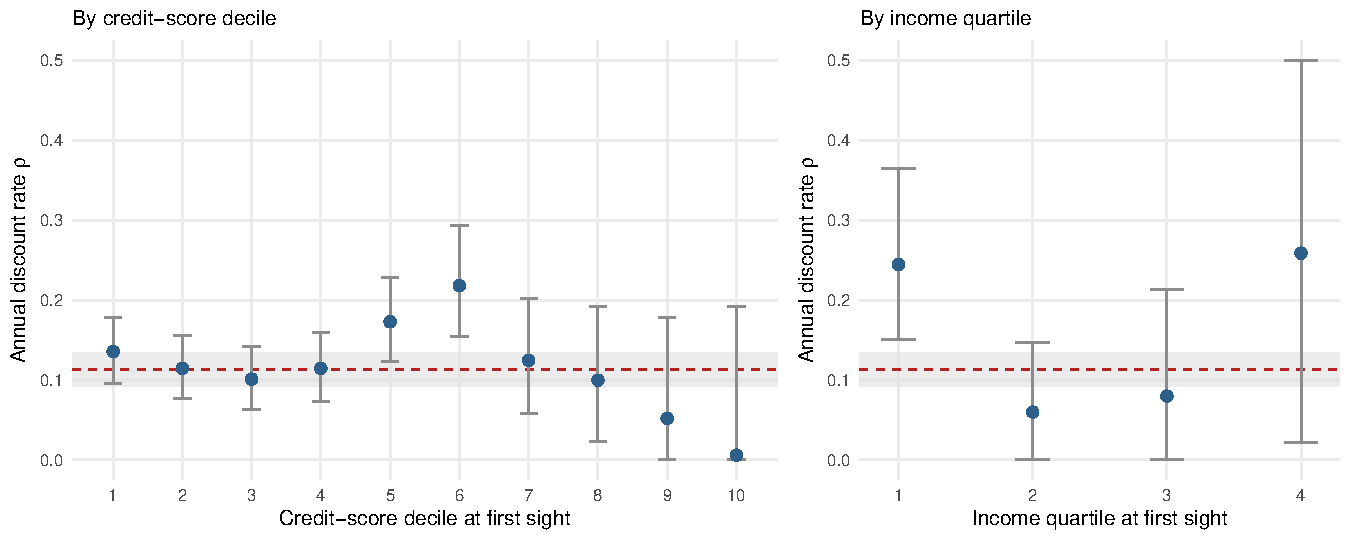
\includegraphics[width=0.8\textwidth,height=0.6\textheight,keepaspectratio]{figures/fig_rho_headline.pdf}
\begin{itemize}\small
\m{$\rho = 0.11$, set $[0.09, 0.13]$, the loan-weighted mean across score deciles of the within-borrower ratios, each mapped through the window formula with the group's own profile and exit hazard.}
\m{The Dobbie--Song experiment, aggregated over its own five-year window, fits best at zero and accepts every rate to $1.2$ at five percent. The experiment fixes the sign of the far-payment weight. The bureau fixes its level.}
\end{itemize}
\backup{bk-experiments}{the experiments}
\end{frame}

\begin{frame}{The level is the bureau's because of where the auto loan sits}
\centering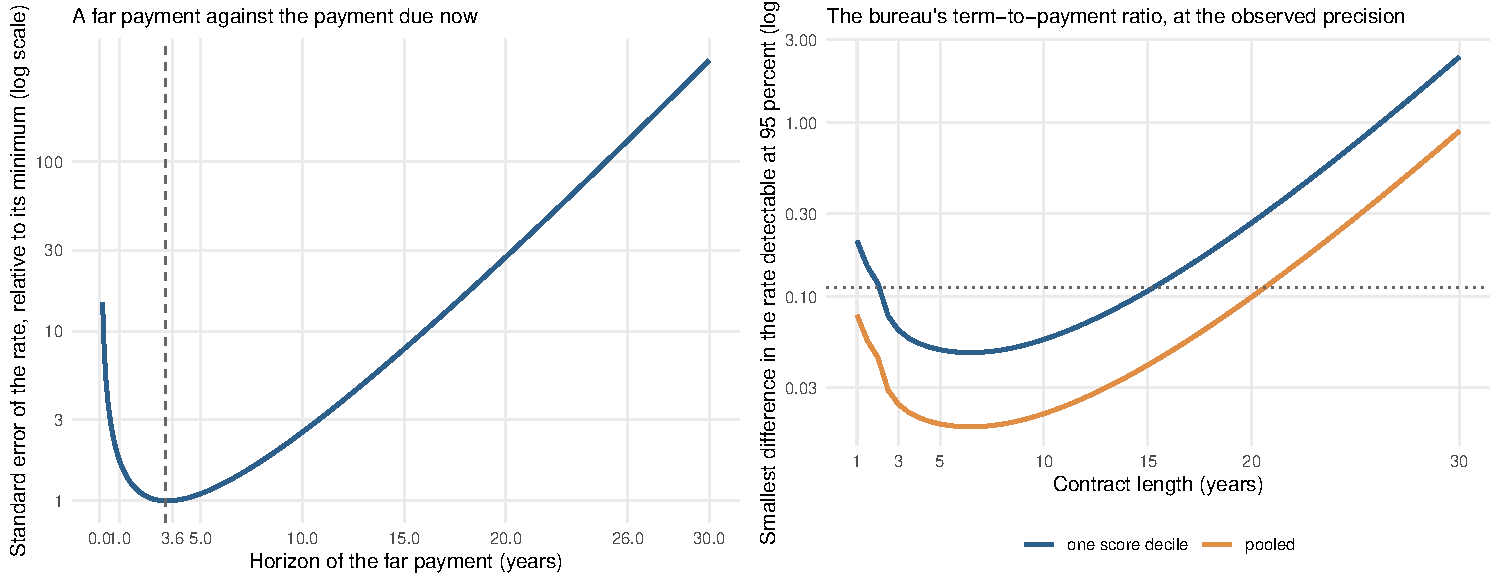
\includegraphics[width=\textwidth,height=0.6\textheight,keepaspectratio]{figures/fig_horizon_power.pdf}
\begin{itemize}\small
\m{A far payment's weight is $\lambda_s e^{-(\rho+h)(s-1)/12}$. Compounding makes it more sensitive to the rate, discounting and survival make it smaller, so the rate's standard error is smallest at $1/(\rho+h)$, $3.3$ years, and $134$ times larger at 26 years.}
\m{A five-year outcome window averages the weight over decisions at which the far payment stands one to five years out, which is why the Dobbie--Song pair bounds the sign and not the level. No design in these data and no published experiment estimates a long-run rate.}
\end{itemize}
\end{frame}

\begin{frame}{The rate across people, from the bureau}
\centering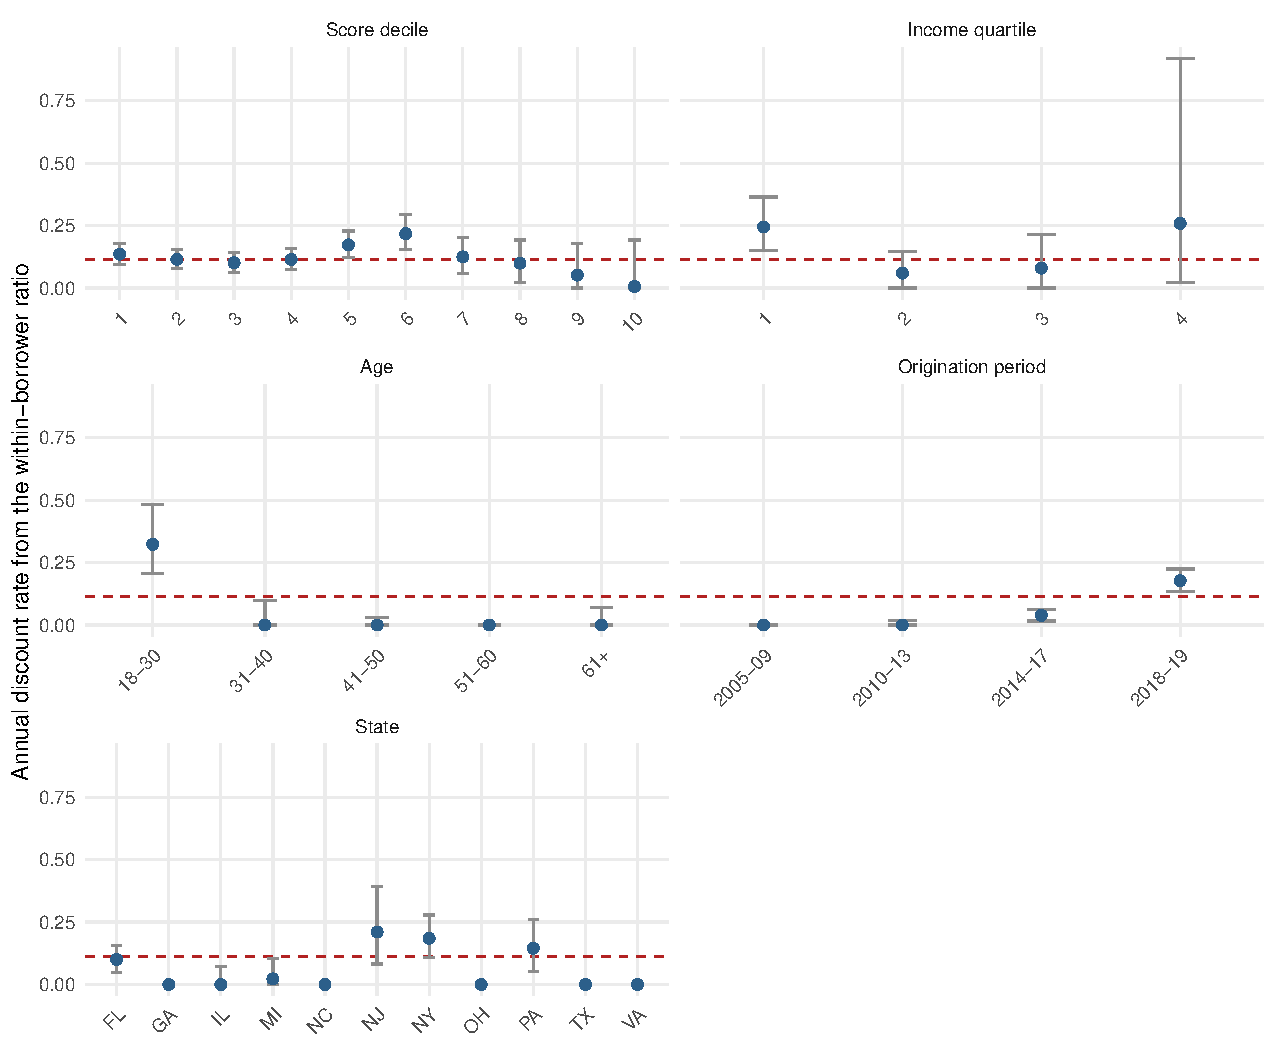
\includegraphics[width=0.9\textwidth,height=0.6\textheight,keepaspectratio]{figures/fig_rho_within.pdf}
\begin{itemize}\small
\m{Within borrower, on 13.5 million borrowers with two or more auto loans (65 million loans), the term response over the payment response at 24 months is mapped through the window formula with each group's own profile and exit hazard.}
\m{Non-monotone in score and income, steepest near the median score and in the bottom income quartile, with sets that include zero in the two top deciles, while default rates fall fifty-fold across the same deciles.}
\end{itemize}
\end{frame}

\begin{frame}{What the bureau adds at population scale}
\centering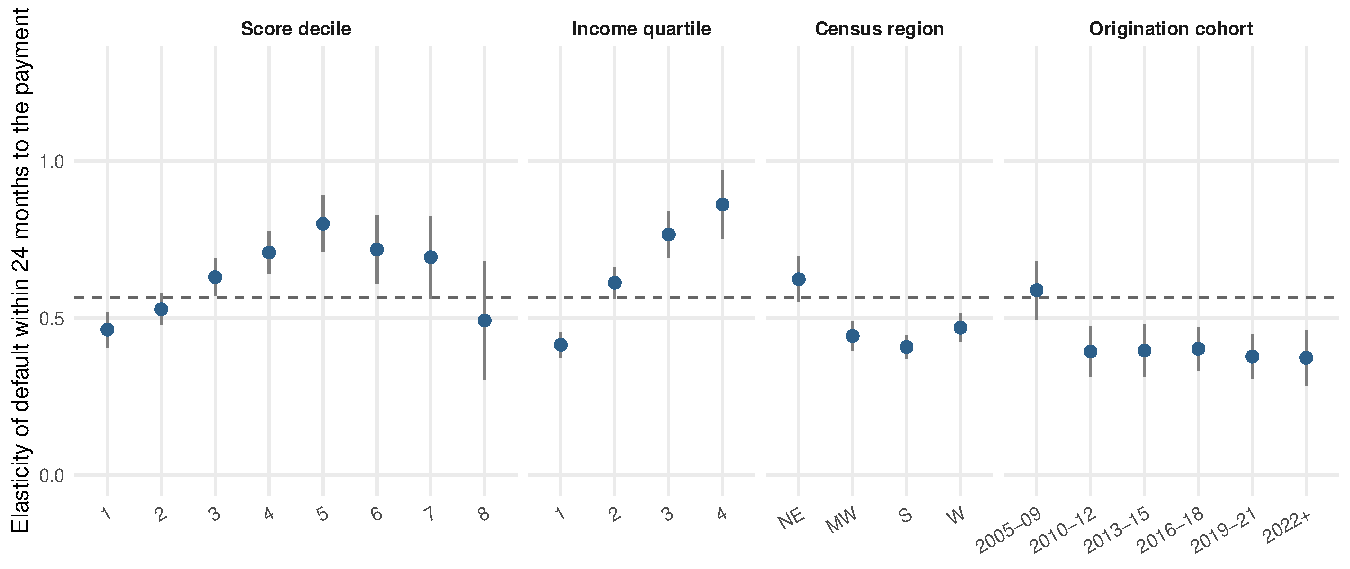
\includegraphics[width=\textwidth,height=0.55\textheight,keepaspectratio]{figures/fig_exposure_groups.pdf}
\begin{itemize}\small
\m{The payment margin at population scale is $0.45$ pooled and $0.44$ within borrower, the same in every cohort from 2010 to 2024, inside the range of the published quasi-experiments' payment responses.}
\m{Its heterogeneity is exposure. The elasticity is $0.41$ in the bottom income quartile and $0.86$ in the top, peaks at the median score, and differs by a factor of two across places.}
\end{itemize}
\backup{bk-bureau}{identification in the bureau}
\end{frame}

\begin{frame}{The data: six loan families, two layers of one bureau}
\centering\resizebox{0.95\textwidth}{!}{\begin{tabular}{lrrrrrr}
\toprule
 & Auto & Credit card & First mortgage & Student & Personal installment & Home equity \\
\midrule
Loans, one-percent panel (millions) & 9.66 & 34.20 & 6.12 & 8.61 & 8.08 & 0.53 \\
Borrowers (millions) & 2.20 & 3.81 & 1.46 & 0.94 & 1.53 & 0.28 \\
Loans, ten-percent archive (millions) & 89.0 &  & 58.2 &  & 73.4 & 4.9 \\
Credit score, median & 698 & 724 & 757 & 653 & 621 & 734 \\
Subprime, below 620 (percent) & 25.0 & 19.7 & 12.0 & 38.2 & 49.6 & 16.4 \\
Monthly income, median (\$) & 3,417 & 3,417 & 4,167 & 2,500 & 2,583 & 4,083 \\
Income below \$2,500 (percent) & 24.0 & 22.1 & 7.2 & 49.1 & 43.7 & 6.8 \\
Scheduled payment, median (\$) &   387 &    29 & 1,263 &    50 &   132 &   359 \\
Ever 90 days past due (percent) & 3.5 & 9.3 & 6.4 & 15.9 & 5.8 & 8.9 \\
Charged off (percent) & 4.9 & 9.7 & 0.2 & 0.8 & 6.3 & 3.1 \\
\bottomrule
\end{tabular}
}
\begin{itemize}\small
\m{A one-percent consumer panel for 2005 to 2025 holds every family, with score, modeled income and lender on each loan. A ten-percent trade archive for 2005 to 2024 holds the within-borrower designs, with 15.5 million auto borrowers who have two or more loans.}
\m{Autos, cards and personal loans reach the households asset prices do not price. A quarter to a half of their borrowers are subprime, and a quarter to a half earn under \$2,500 a month.}
\end{itemize}
\end{frame}


\begin{frame}{Parallel laboratories}
\centering\footnotesize
\resizebox{\textwidth}{!}{\begin{tabular}{@{}p{2.2cm}p{3.1cm}p{1.9cm}p{3.8cm}p{3.8cm}@{}}
\toprule
Loan type & Coverage & Horizon & Instrument & Delivers \\
\midrule
Auto loans & The low end of income and score; 7.6 million loans & 1--6 years & Payment and term margins in zip-month cells; within borrower; deficiency contrast & The payment margin at scale and its exposure heterogeneity; the within-borrower reading: 0.01 pooled, 0.09 across deciles, no gradient \\
Credit cards & The same low end & Months to 4 years & Issuer-set minimum-payment formula and rate changes & The revolving extension; the formula design \\
First mortgages & Homeowners & Up to 30 years & House prices by cohort within zip-quarter; contract-fixed resets; state recourse & The equity margin and walk-away signatures; the reset facts; the penalty channel \\
Student loans & Post-secondary borrowers & 10--25 years & The 2023 statutory resumption & Auto default does not respond to an unenforced bill \\
\bottomrule
\end{tabular}}
\begin{itemize}\small
\m{Autos and cards reach the households that asset prices do not price and laboratories do not sample, and they supply the weight of the evidence. Mortgages supply the long horizons and the strongest instruments.}
\end{itemize}
\end{frame}


\begin{frame}{What the contract's length measures in the bureau}
\[ \underbrace{\textstyle\sum_{t \le K}\omega_t\, D(T-t)\, Q_{T-t}\, \lambda}_{\text{preference channel}} \;-\; \underbrace{\textstyle\sum_{t \le K}\omega_t\, \tfrac{\kappa_B}{\bar y}(1+r)^{-(T-t)}}_{\text{penalty channel}} \;+\; \underbrace{\mathbf{1}[K = T]\,(1 - D_T)\,\bar p_{T+}}_{\text{exposure}} \]
\begin{itemize}
\m{A longer contract at a fixed payment adds far payments, raises the balance and with it a penalty that scales with the balance, and adds months of exposure. Across borrowers it also changes who selects which length.}
\m{The preference channel is bounded by one in units of the payment response, so a measured ratio above one is outside it at any rate. The deficiency-judgment contrast measures the penalty channel, a fixed window removes exposure, and holding the borrower fixed removes selection.}
\m{A rate comes from the contract's length only with the borrower held fixed and the penalty channel decayed, which is the within-borrower design at 24 months.}
\end{itemize}
\end{frame}

\begin{frame}{The across-borrower term margin, adjusted rung by rung}
\centering\resizebox{0.95\textwidth}{!}{\begin{tabular}{llrrrrrr}
\toprule
Outcome & $\psi$ & $\varepsilon_m$ & $\varepsilon_T$ & Raw $R$ ($\rho$) & + penalty ($\rho$) & + selection $R$ (s.e.) & $\rho$ [95\% set] \\
\midrule
Charge-off within twelve months & 1.0 & 0.45 (0.02) & 0.01 (0.05) & 0.01 (1.06) & 0.81 (0.00) & 0.39 (0.31) & 0.04 [0.00, $\infty$] \\
Charge-off within twelve months & 2.5 & 0.45 (0.02) & 0.01 (0.05) & 0.01 (1.06) & 2.01 (0.00) & 1.59 (0.73) & 0.00 [0.00, 0.32] \\
90-day delinquency within twelve months & 1.0 & 0.35 (0.02) & -0.27 (0.04) & -0.77 ($\infty$) & 0.25 (0.19) & -0.29 (0.39) & $\infty$ [0.00, $\infty$] \\
90-day delinquency within twelve months & 2.5 & 0.35 (0.02) & -0.27 (0.04) & -0.77 ($\infty$) & 1.78 (0.00) & 1.24 (0.92) & 0.00 [0.00, $\infty$] \\
\midrule
Rule-based experiments, Dobbie--Song pair (for reference) & & & & & & & best fit 0.00; [0.00, 1.20] (5\%), [0.00, 2.84] (1\%) \\
\bottomrule
\end{tabular}
}
\begin{itemize}\small
\m{The term response over the payment response within twelve months, across borrowers on 7.6 million auto loans. Raw, the far payments have no weight. The two corrections the theory names, the penalty channel ($+0.36$ from the deficiency contrast) and selection into term ($-0.19$ from the within-borrower design), are each measured once.}
\m{Corrected, the ratio is $0.39$ ($0.31$), which the window formula maps to $\rho = 0.04$ with a set that spans the grid. The within-borrower ratio is the estimate, and the ladder checks the size of the penalty channel it leaves unsubtracted.}
\end{itemize}
\end{frame}


\begin{frame}{The run-off of the payment margin validates the stopping model}
\centering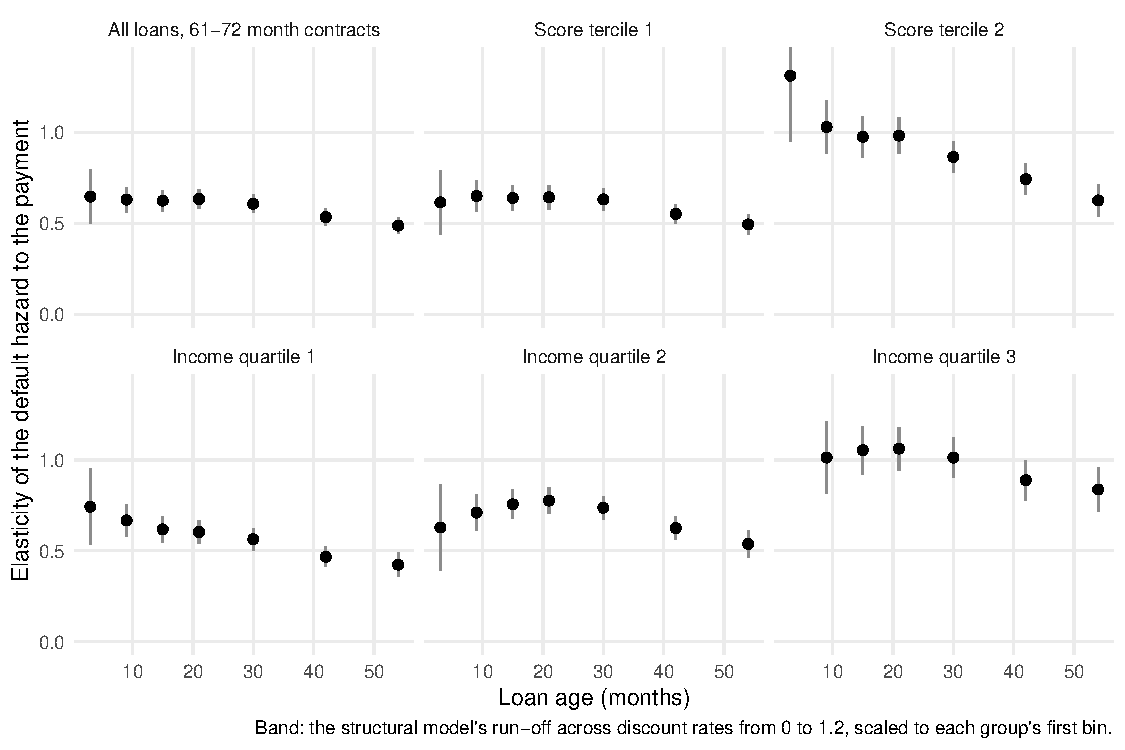
\includegraphics[width=0.9\textwidth,height=0.55\textheight,keepaspectratio]{figures/fig_runoff_profiles.pdf}
\begin{itemize}\small
\m{The payment elasticity is flat for three years and then falls to three quarters of its level, the same shape in every group.}
\m{The structural model, calibrated to the default rate, produces this shape at every discount rate under an i.i.d.\ or a persistent income process, because the default option sets the weight on far payments. The run-off is evidence for the model and is not mapped to a rate.}
\end{itemize}
\backup{bk-runoff}{the model's run-off}
\end{frame}

\begin{frame}{The rate varies non-monotonically across groups}
\centering\resizebox{0.68\textwidth}{!}{\begin{tabular}{llrrrrrrr}
\toprule
Dimension & Group & Loans & $R_{24}$ (s.e.) & $\lambda_{2}$ & $\lambda_{60}$ & $h$ & $\rho$ & 95\% set \\
\midrule
All &  & 59,155,190 & 0.55 (0.01) & 0.89 & 0.35 & 0.19 & 0.02 & [0.01, 0.04] \\
Score decile & 1 & 5,754,666 & 0.53 (0.03) & 0.89 & 0.40 & 0.13 & 0.14 & [0.10, 0.18] \\
Score decile & 2 & 5,784,547 & 0.50 (0.02) & 0.89 & 0.39 & 0.17 & 0.11 & [0.08, 0.16] \\
Score decile & 3 & 5,819,449 & 0.47 (0.02) & 0.89 & 0.37 & 0.19 & 0.10 & [0.06, 0.14] \\
Score decile & 4 & 5,837,786 & 0.44 (0.02) & 0.89 & 0.36 & 0.20 & 0.11 & [0.07, 0.16] \\
Score decile & 5 & 5,840,925 & 0.37 (0.03) & 0.89 & 0.34 & 0.20 & 0.17 & [0.12, 0.23] \\
Score decile & 6 & 5,895,688 & 0.32 (0.03) & 0.88 & 0.32 & 0.20 & 0.22 & [0.15, 0.29] \\
Score decile & 7 & 5,958,258 & 0.39 (0.04) & 0.88 & 0.31 & 0.21 & 0.12 & [0.06, 0.20] \\
Score decile & 8 & 6,024,937 & 0.40 (0.04) & 0.88 & 0.29 & 0.21 & 0.10 & [0.02, 0.19] \\
Score decile & 9 & 6,094,315 & 0.44 (0.06) & 0.88 & 0.28 & 0.21 & 0.05 & [0.00, 0.18] \\
Score decile & 10 & 6,144,619 & 0.49 (0.10) & 0.88 & 0.26 & 0.20 & 0.01 & [0.00, 0.19] \\
Income quartile & 1 & 1,417,320 & 0.34 (0.05) & 0.89 & 0.38 & 0.18 & 0.24 & [0.15, 0.36] \\
Income quartile & 2 & 1,464,021 & 0.52 (0.05) & 0.89 & 0.37 & 0.19 & 0.06 & [0.00, 0.15] \\
Income quartile & 3 & 1,507,500 & 0.45 (0.07) & 0.88 & 0.32 & 0.21 & 0.08 & [0.00, 0.21] \\
Income quartile & 4 & 1,525,715 & 0.27 (0.12) & 0.88 & 0.29 & 0.20 & 0.26 & [0.02, 0.92] \\
\bottomrule
\end{tabular}
}
\begin{itemize}\small
\m{By score decile the rate runs from $0.01$ to $0.22$, with sets that contain the mean in eight deciles. By income quartile it is $0.24$, $0.06$, $0.08$ and $0.26$. The ratios themselves differ little, $0.53$ at the bottom decile and $0.49$ at the top.}
\m{Heterogeneity in default is in the level of the margin, exposure. The rate is steepest near the median score and in the bottom income quartile, and nowhere rises with the group's default rate.}
\end{itemize}
\end{frame}

\begin{frame}{The rate by subgroup, from the one experiment that reports both arms by subgroup}
\centering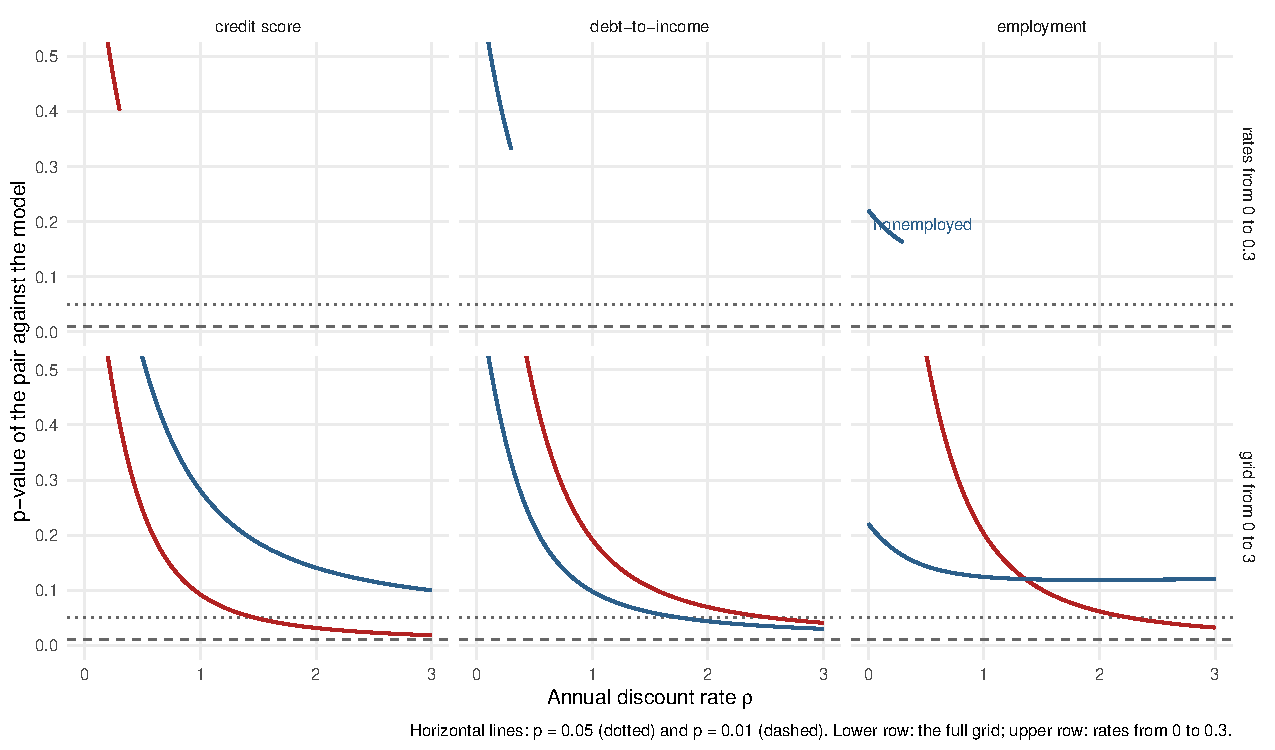
\includegraphics[width=\textwidth,height=0.5\textheight,keepaspectratio]{figures/fig_rho_subgroups.pdf}
\begin{itemize}\small
\m{In Dobbie--Song the best fit lies between zero and $0.20$ in every subgroup, no reference rate is rejected at five percent, and the two halves of each split do not differ ($p = 0.64$, $0.84$ and $0.21$ for the ratios).}
\m{The axes along which default differs most, credit score and leverage, are not axes along which the rate differs.}
\end{itemize}
\end{frame}

\begin{frame}{The population term margin is a selection gradient in the score}
\centering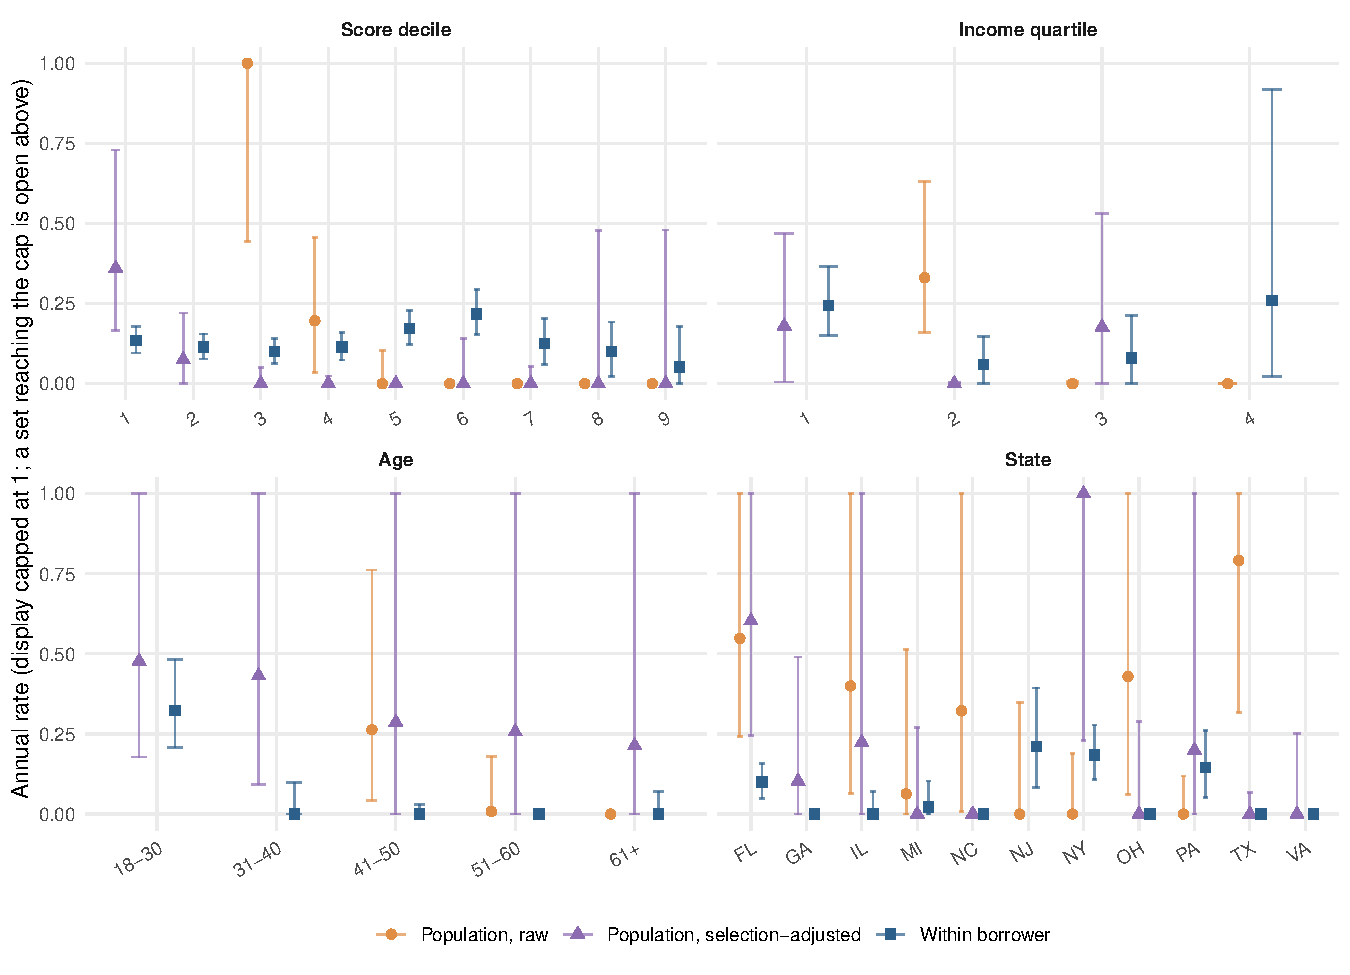
\includegraphics[width=\textwidth,height=0.58\textheight,keepaspectratio]{figures/fig_het_agreement.pdf}
\begin{itemize}\small
\m{Pooled, the population ratio is $0.25$ against $0.55$ within borrower. By decile it rises from $-0.95$ to $4.45$ while the within-borrower ratio stays between $0.32$ and $0.53$, because lenders screen risky borrowers with short terms and safe borrowers choose long ones.}
\m{The population step buys exposure with power at every resolution and the selection gradient at 46 points of the score distribution. It does not buy a rate by group.}
\end{itemize}
\end{frame}

\begin{frame}{The geography of exposure follows income}
\centering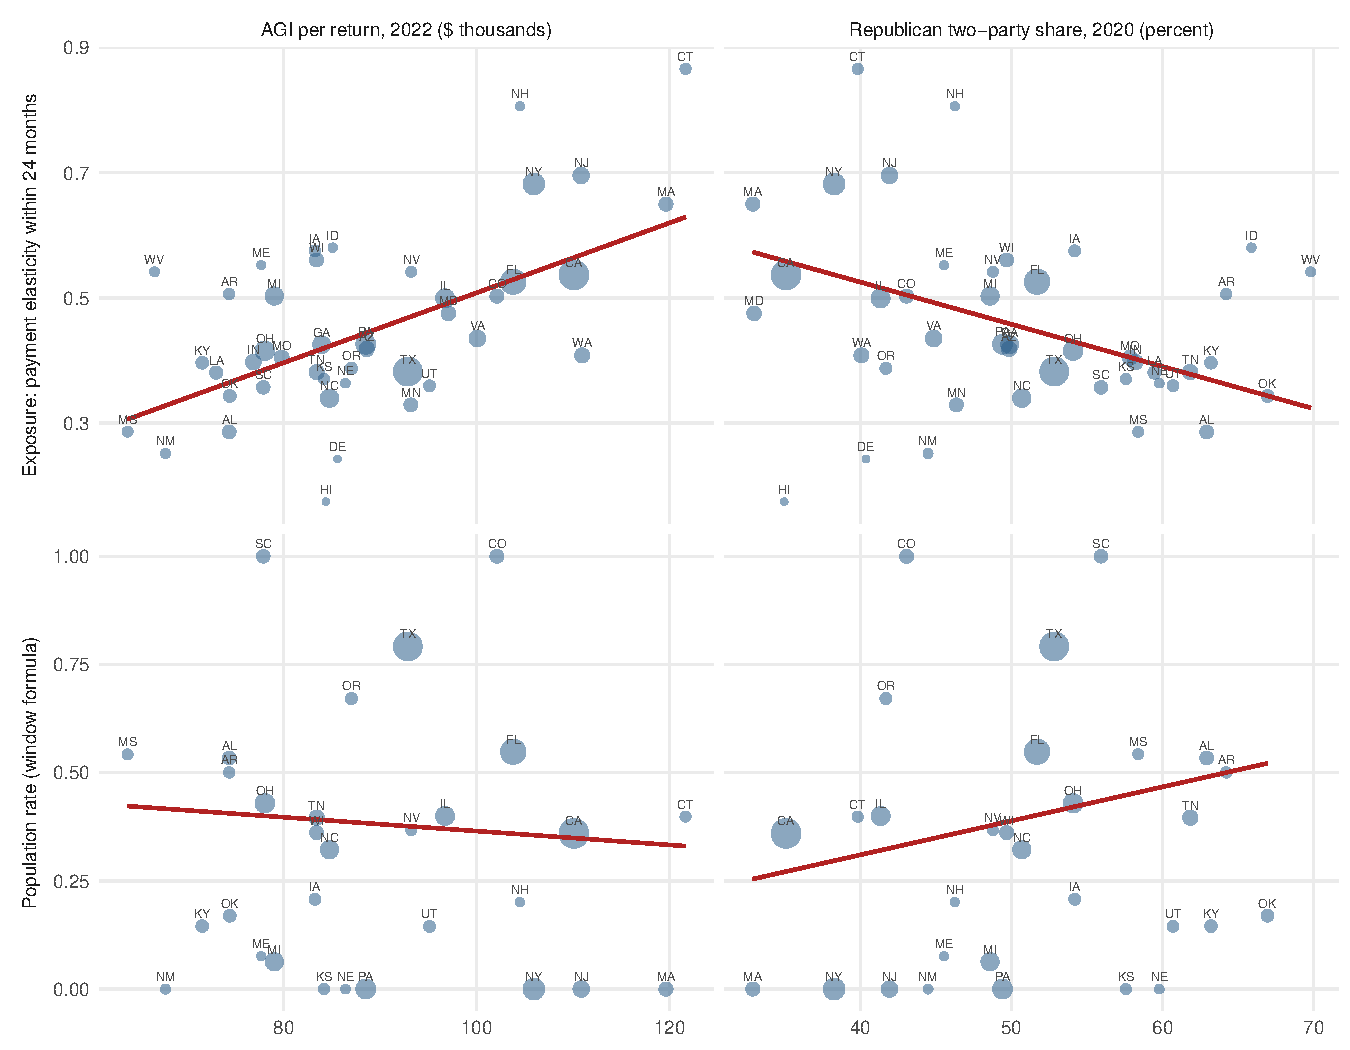
\includegraphics[width=\textwidth,height=0.42\textheight,keepaspectratio]{figures/fig_geo_correlates.pdf}
\begin{itemize}\small
\m{Across 91 zip-code areas exposure runs from $0.33$ to $0.67$ (tenth to ninetieth percentile). One standard deviation of income per return raises it by $0.07$ across states; one of the Republican share lowers it by $0.06$.}
\m{With composition held fixed, the vote's gradient is zero and income's survives only across states. The political map of default is an income map, and not a map of the rate, whose ratio cancels the level of default by construction.}
\m{A rate by place from place-by-score-tercile cells, the place fixed at the borrower's first loan. Florida 0.19, New York 0.24, Pennsylvania 0.23, New Jersey 0.38 on the deciles' footing; twenty-two southern and midwestern states have every cell above the ceiling, a bound at zero.}
\end{itemize}
\end{frame}

\begin{frame}{First mortgages: the equity response has the signatures of a walk-away}
\centering\resizebox{0.95\textwidth}{!}{\begin{tabular}{lrrrrrr}
\toprule
Sample & Loans & Events & Base & House price ($\varepsilon$) & Payment ($\varepsilon$) & Ratio \\
\midrule
All & 1,863,861 & 191,581 & 0.88 & -2.232 (0.089) [-2.54] & 1.308 (0.039) [1.49] & -1.71 (0.07) \\
States without deficiency judgments & 580,429 & 54,314 & 0.83 & -2.275 (0.085) [-2.74] & 0.955 (0.062) [1.15] & -2.38 (0.16) \\
States with deficiency judgments & 1,283,432 & 137,267 & 0.90 & -2.229 (0.140) [-2.48] & 1.447 (0.042) [1.61] & -1.54 (0.09) \\
Loan age 0--3 years & 1,340,631 & 64,010 & 0.75 & -4.434 (0.168) [-5.90] & 1.380 (0.045) [1.84] & -3.21 (0.16) \\
Loan age 3--7 years & 949,582 & 92,264 & 1.24 & -3.569 (0.131) [-2.88] & 1.569 (0.072) [1.27] & -2.27 (0.10) \\
Loan age 7 years and more & 477,513 & 35,307 & 0.61 & -0.646 (0.045) [-1.07] & 0.833 (0.025) [1.37] & -0.78 (0.05) \\
2008--12 & 1,353,418 & 132,763 & 1.51 & -4.667 (0.202) [-3.09] & 1.996 (0.082) [1.32] & -2.34 (0.12) \\
2013--18 & 585,217 & 40,866 & 0.47 & -0.591 (0.046) [-1.26] & 0.678 (0.019) [1.45] & -0.87 (0.06) \\
\bottomrule
\end{tabular}
}
\begin{itemize}\small
\m{1.86 million thirty-year mortgages of 2000 to 2012, followed quarterly to the first 90-day delinquency, within zip-by-quarter and origination-year cells. A ten percent price fall raises the hazard by a quarter.}
\m{The response is stronger where the lender cannot pursue the balance ($-2.7$ against $-2.5$), falls with loan age ($-5.9$ to $-1.1$) and is convex in negative equity. In the model with a house the equity-to-payment ratio is $-0.92$ to $-1.09$ at every rate, because a borrower with positive equity sells rather than defaults.}
\end{itemize}
\end{frame}

\begin{frame}{Timing variation inside the bureau: the adjustable-rate resets}
\centering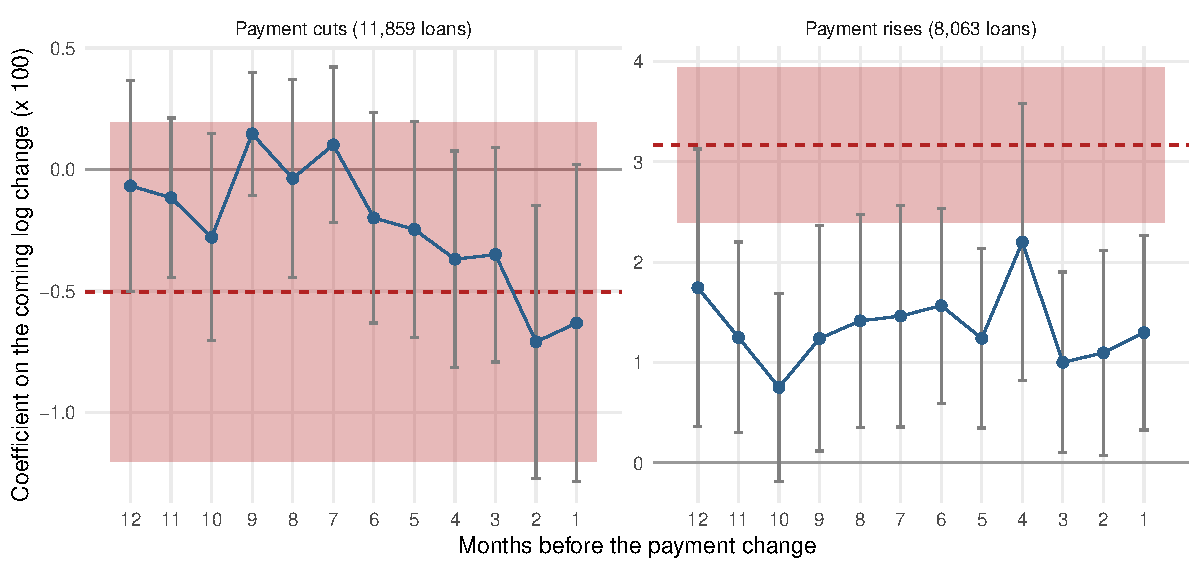
\includegraphics[width=0.9\textwidth,height=0.48\textheight,keepaspectratio]{figures/fig_arm_anticipation.pdf}
\begin{itemize}\small
\m{The panel has no contract flag, so the amortization identity recovers the note rate from the balance path. Of 88,151 payment changes at hybrid reset ages, 9,224 are rate changes, from 6.0 to 3.2 percent at the median.}
\m{At the cut, within loan and vintage month, the response is not distinguishable from zero or from the elasticity of record (1,066 events). Delinquency is higher before a larger coming cut in every sample. Under Proposition 3 the response before a change has the sign of the response at it, so the profile is not a discount function.}
\end{itemize}
\end{frame}

\begin{frame}{Timing variation inside the bureau: the 2023 student-loan resumption}
\centering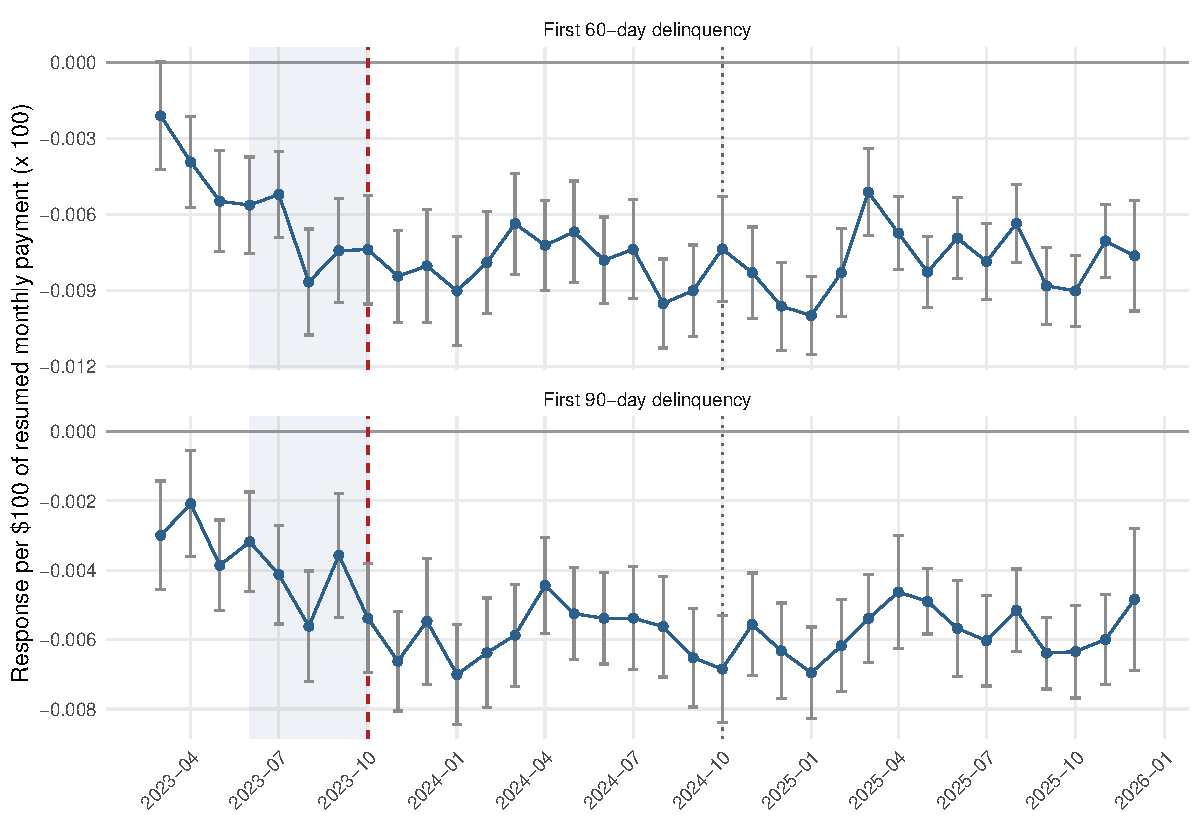
\includegraphics[width=0.8\textwidth,height=0.5\textheight,keepaspectratio]{figures/fig_student_profile.pdf}
\begin{itemize}\small
\m{A bill on another account, with its date fixed by statute four months ahead and its size fixed by the loan, for 438,311 holders with 743,487 auto loans and 17,711 first 90-day events. The response per \$100 of bill is negative in every month, before the statute as well as after, which is composition rather than a response.}
\m{Half of the bills went unpaid and none were reported delinquent for a year. A payment that need not be made has no weight in Proposition 3, so the zero is the model's zero.}
\end{itemize}
\end{frame}


\begin{frame}{Contributions}
\begin{itemize}\small
\m{\textbf{Theory.} A sufficient statistic for the discount function from default responses to payments at two dates. Three theorems on its limits (the premium, beliefs, the contract's length). A window formula that assigns each default to its own decision month, and a precision result that says at which horizon a rate can be estimated.}
\m{\textbf{The rate.} $0.11$ over the horizon of a contract, from two loans of the same borrower, varying non-monotonically with score and income, steepest near median scores and at the lowest incomes, with a gradient in age. The published experiments accept it and, run over windows of years at horizons of four to twenty-six years, fix its sign and not its level.}
\m{\textbf{Default is strategic.} The cost of default rises with the balance owed ($+0.36$ on the term response where the balance cannot be pursued, $+3.9$ on mortgages without recourse), and the equity response of mortgage default is a walk-away, stronger without recourse and convex in negative equity.}
\m{\textbf{Exposure at population scale.} The payment elasticity runs from $0.41$ to $0.86$ across income quartiles and by a factor of two across places, follows income rather than the vote, and the population term margin is the Hertzberg et al.\ selection pattern at 46 points of the score distribution.}
\end{itemize}
\end{frame}

\begin{frame}{What is next}
\begin{itemize}
\m{The adjustable-rate resets in the bureau are found and do not deliver the rate, because the index moved by less than $0.2$ points in 2010 to 2013 and delinquency is higher before a coming cut in every sample, a sign no discount function produces.}
\m{The October 2023 student-loan resumption, a statutory bill on another account, moved nothing, because half of the bills went unpaid and none were reported delinquent for a year.}
\m{HAMP step-ups, card promotional expirations and forbearance exits are queued. Each moves a payment at a known date at a fixed balance, in the panel, with score, income and lender on every loan.}
\end{itemize}
\label{main-end}
\end{frame}

%%%%%%%%%%%%%%%%%%%%%%%%%%%% BACKUP %%%%%%%%%%%%%%%%%%%%%%%%%%%%
\begin{frame}[plain]\centering\Large Backup\end{frame}

\begin{frame}[label=bk-theory]{The propositions}
\begin{itemize}\small
\m{Interior default at every horizon. The borrower who continues buys one period of standing plus the option to reconsider, and committed-repayment comparisons degenerate.}
\m{Sensitivities. $\partial p_1/\partial m_s = f(y^*)\,\delta^{s-1} Q_s\, \mathbb{E}[u'(y-m_s)\mid y>y_s^*]/\Delta u'_1$.}
\m{The discount curve is identified pointwise from a menu of payment perturbations with survival measured, and the exponential null is testable with three horizons.}
\m{Exact aggregation. A pooled estimate is a sensitivity-weighted average of type-level statistics, with weights equal to each type's mass at its own margin.}
\end{itemize}\backto
\end{frame}

\begin{frame}[label=bk-limits]{The theorems on limits}
\begin{itemize}\small
\m{\textbf{Theorem.} With $D(k)=\beta\delta^k$ and the profile $\lambda_s$, every ratio of default responses depends on $(\beta,\lambda_s)$ through $\beta\lambda_s$. Payment-timing experiments identify $\delta$ and $\beta\lambda_s$ and neither factor alone.}
\m{\textbf{Corollary.} A liquid-versus-illiquid comparison at one date identifies $\lambda$ (Indarte's pair, $\lambda \approx 0.2$), and then $\beta$ follows.}
\m{\textbf{Proposition.} Subjective survival $\tilde Q$ multiplies $D$. The identified object is $D\,\tilde Q/Q$, fixed by measuring $Q$.}
\m{\textbf{Proposition.} The term response is the preference channel minus the balance-scaled penalty plus exposure, and a ratio above one is outside the preference channel at any rate.}
\end{itemize}\backto
\end{frame}

\begin{frame}[label=bk-experiments]{The experiments as payment paths}
\centering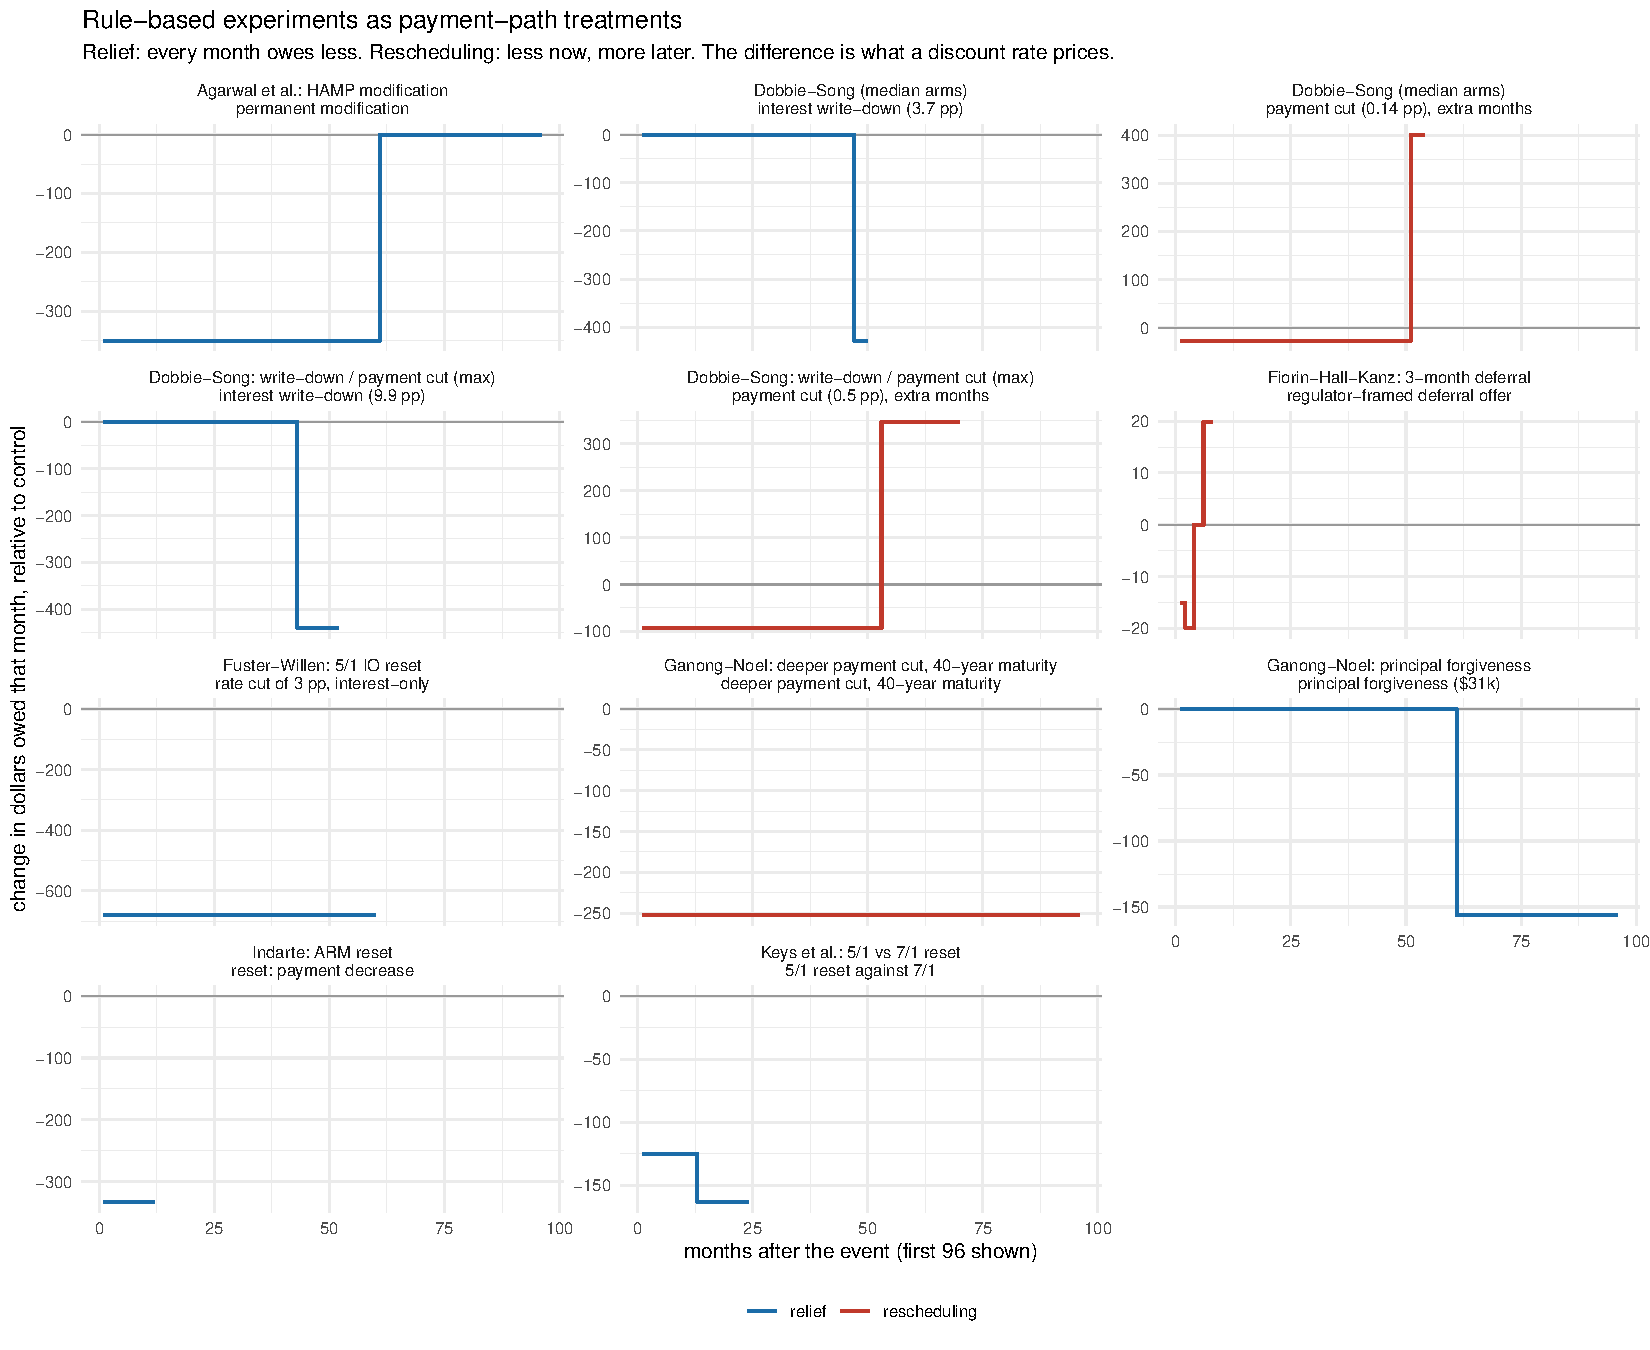
\includegraphics[width=0.9\textwidth,height=0.62\textheight,keepaspectratio]{figures/fig_ledger_paths.pdf}
\begin{itemize}\small\m{A relief owes less in every month. A rescheduling owes less now and more later. The distinction is what a discount rate prices.}\end{itemize}\backto
\end{frame}

\begin{frame}{What each pair says}
\centering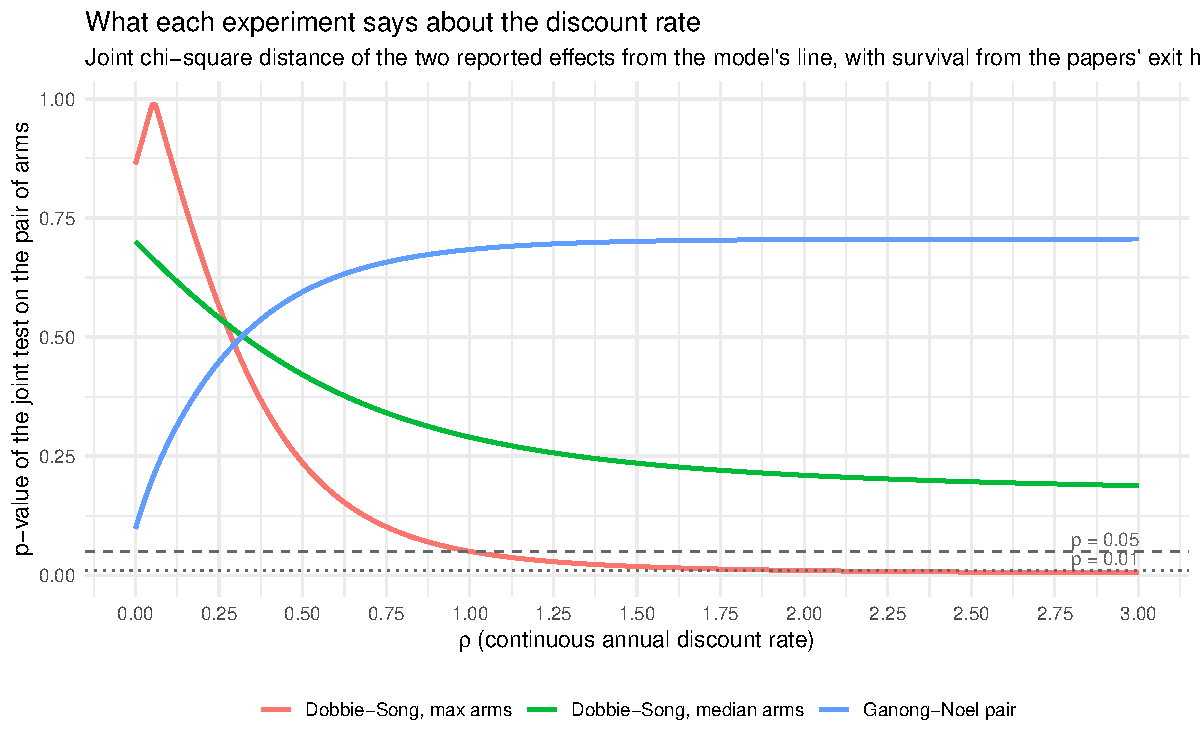
\includegraphics[width=0.75\textwidth,height=0.62\textheight,keepaspectratio]{figures/fig_ledger_rho.pdf}
\begin{itemize}\small\m{Dobbie--Song, over its own five-year window, fits best at zero and accepts $[0, 1.20]$ at five percent and $[0, 2.84]$ at one percent. Read at a single decision date the sets would end at $0.03$ and $0.08$. Ganong--Noel is nearly flat over 26 years and rejects nothing. Indarte's pair identifies $\lambda$.}\end{itemize}\backto
\end{frame}

\begin{frame}{The near-horizon response across settings, and $\lambda$}
\centering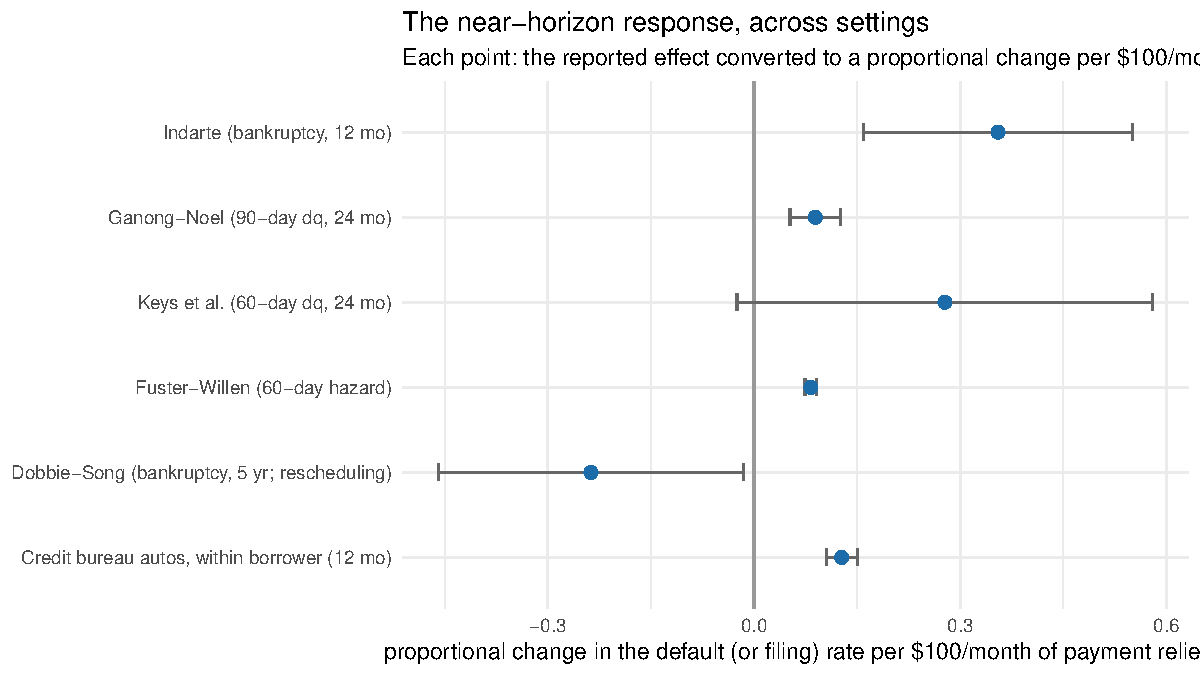
\includegraphics[width=0.7\textwidth,height=0.4\textheight,keepaspectratio]{figures/fig_ledger_near.pdf}\\
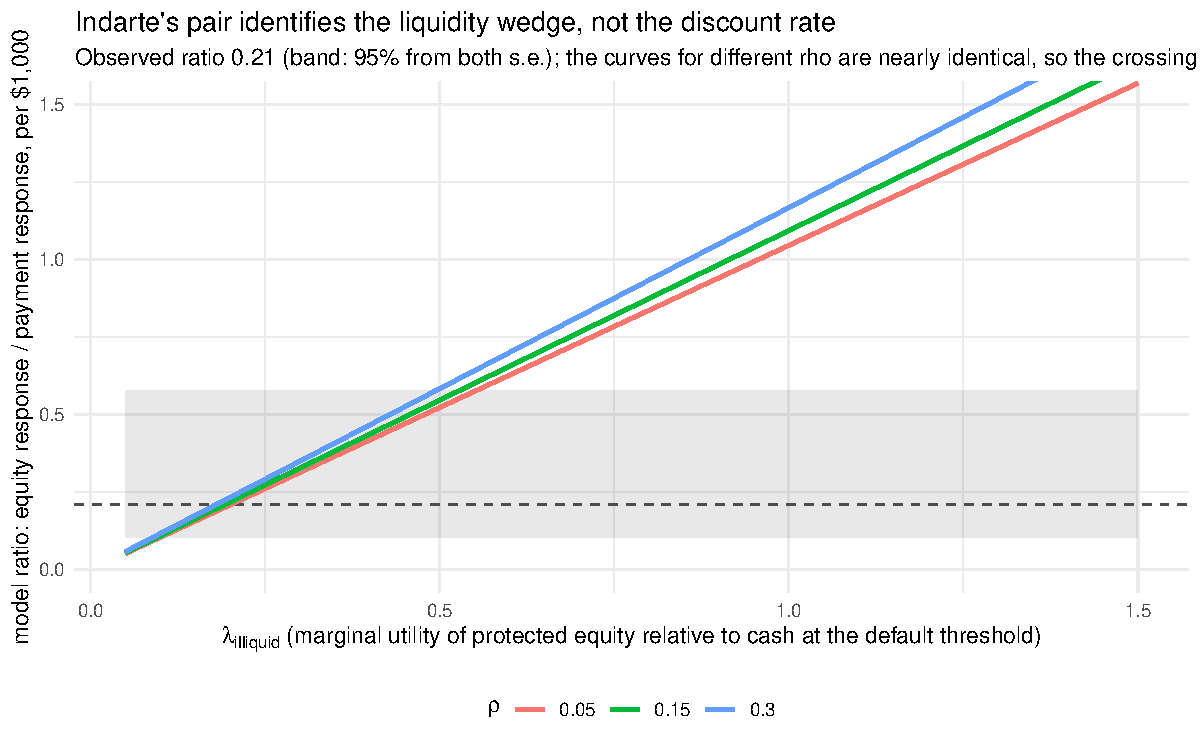
\includegraphics[width=0.7\textwidth,height=0.4\textheight,keepaspectratio]{figures/fig_ledger_lambda.pdf}\backto
\end{frame}

\begin{frame}[label=bk-bureau]{The payment margin is a stable parameter}
\centering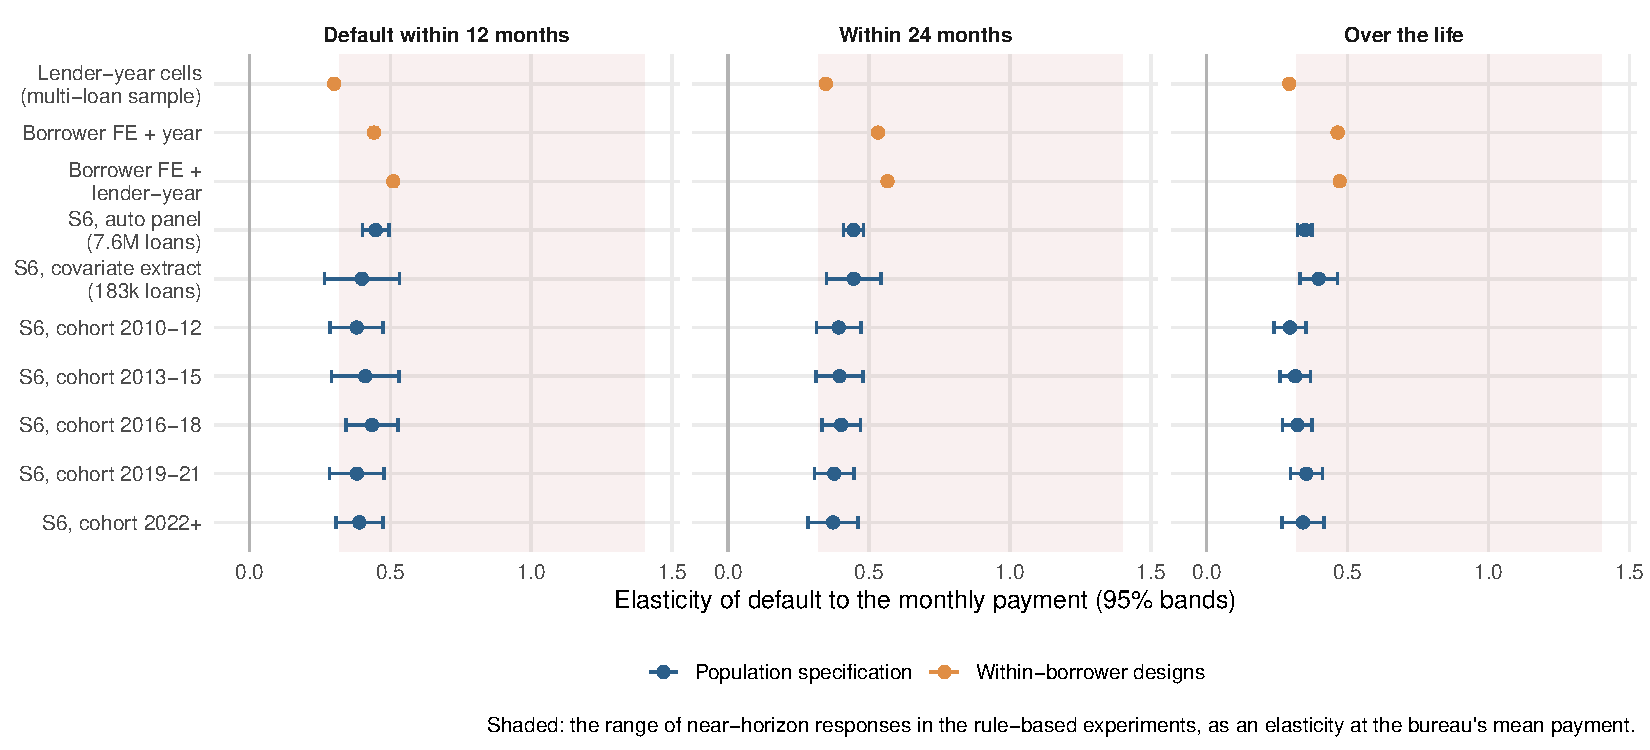
\includegraphics[width=\textwidth,height=0.62\textheight,keepaspectratio]{figures/fig_stability.pdf}
\begin{itemize}\small\m{Within-borrower designs, the population specification on the panel, and every cohort lie between $0.3$ and $0.6$, inside the range of the published payment responses.}\end{itemize}\backto
\end{frame}

\begin{frame}{The specification search}
\centering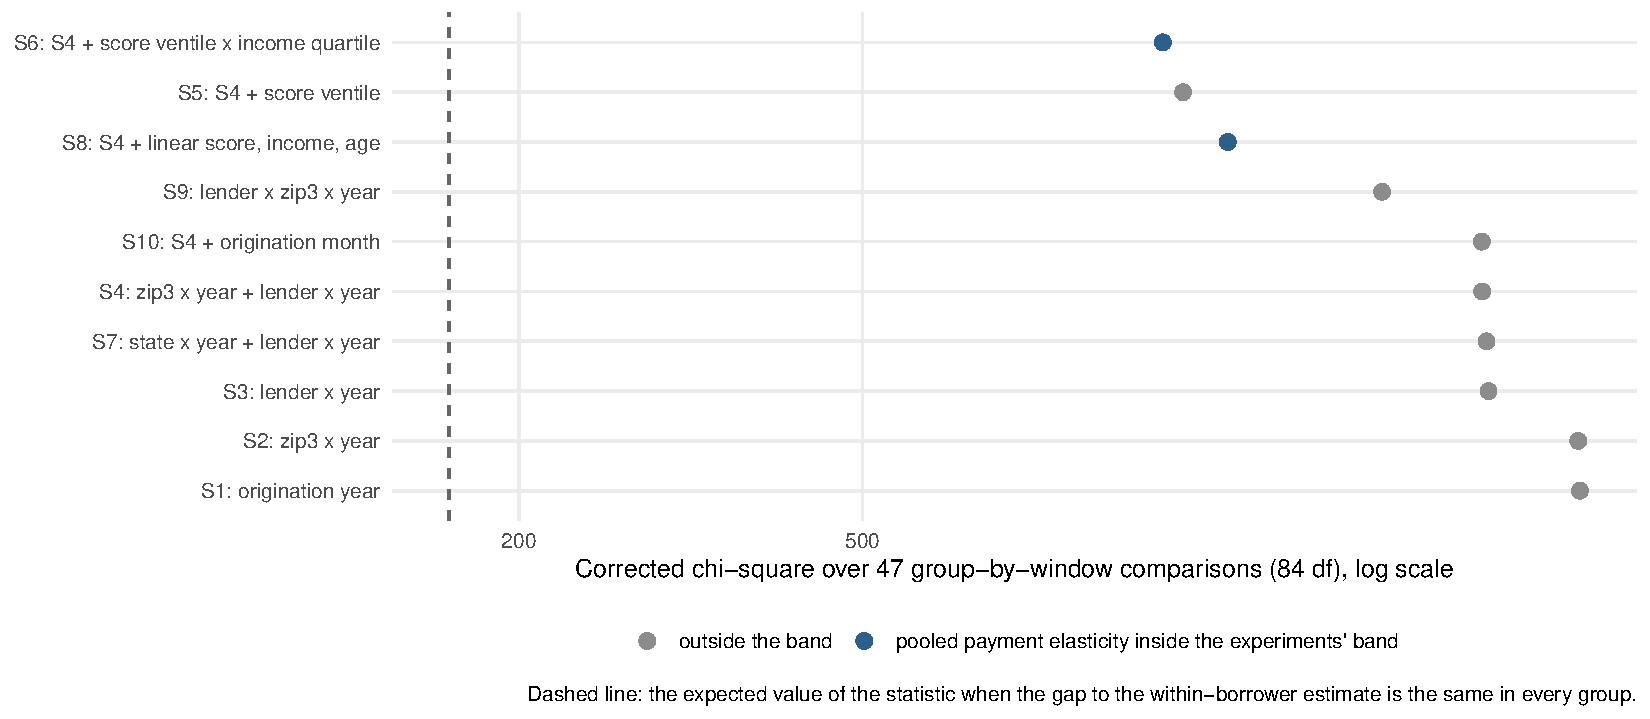
\includegraphics[width=\textwidth,height=0.6\textheight,keepaspectratio]{figures/fig_spec.pdf}
\begin{itemize}\small\m{Ten candidates scored on 47 group-by-window comparisons against within-borrower estimates. One reproduces them in every group with a constant gap.}\end{itemize}\backto
\end{frame}

\begin{frame}{The gap to the within-borrower estimate, by group}
\centering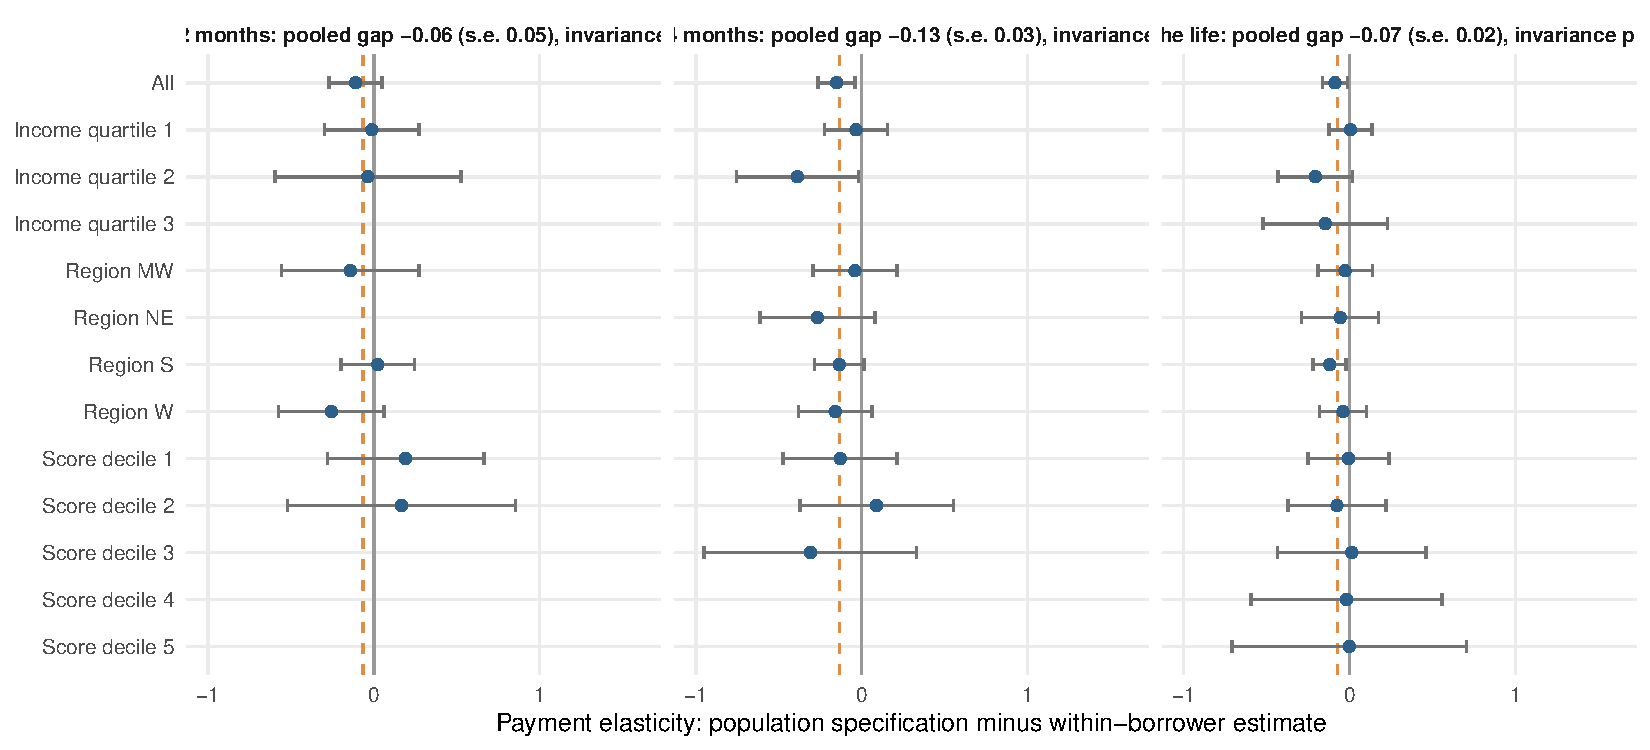
\includegraphics[width=\textwidth,height=0.62\textheight,keepaspectratio]{figures/fig_gap.pdf}\backto
\end{frame}

\begin{frame}{The term margin has two channels}
\centering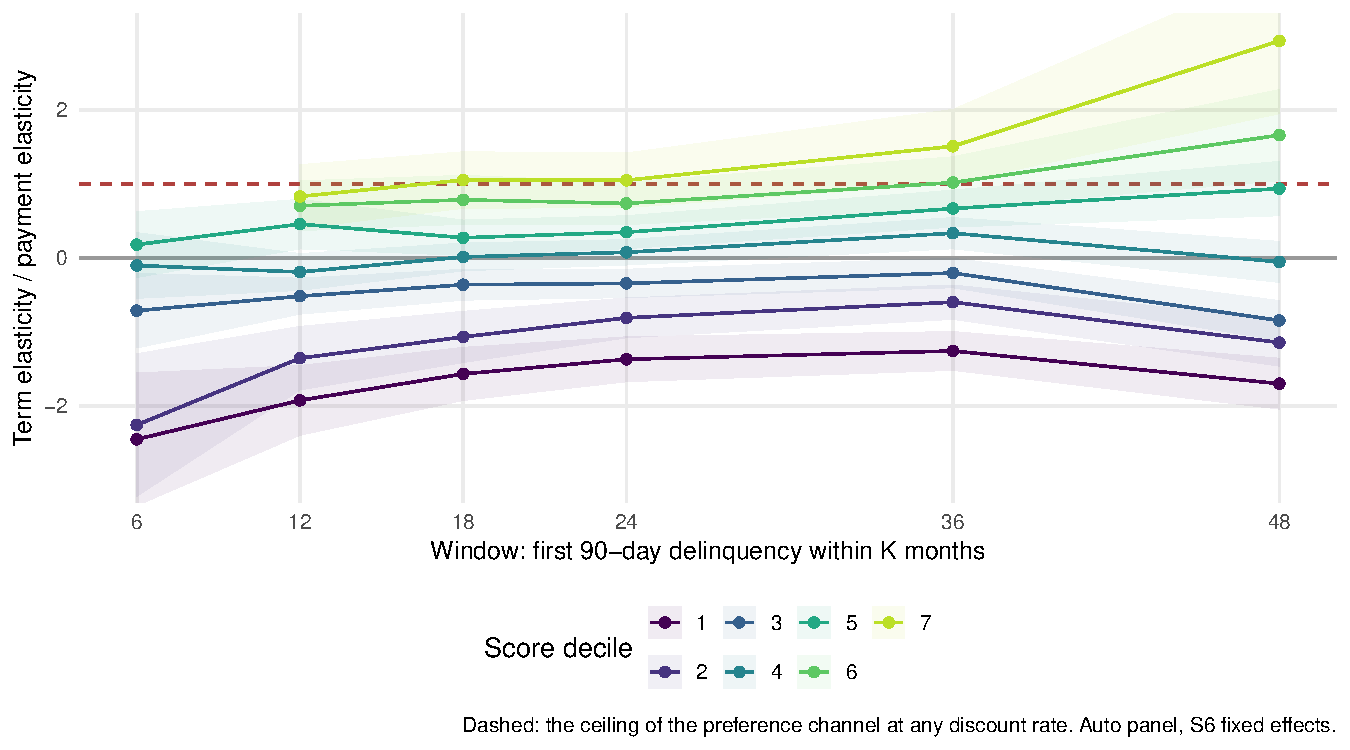
\includegraphics[width=0.8\textwidth,height=0.55\textheight,keepaspectratio]{figures/fig_termmargin.pdf}
\begin{itemize}\small\m{At a fixed payment a longer contract lowers early delinquency for low scores and raises it for high scores. Values above one are outside the preference channel, and the deficiency rules confirm the penalty channel.}\end{itemize}\backto
\end{frame}

\begin{frame}{Person, place, and the penalty base}
\centering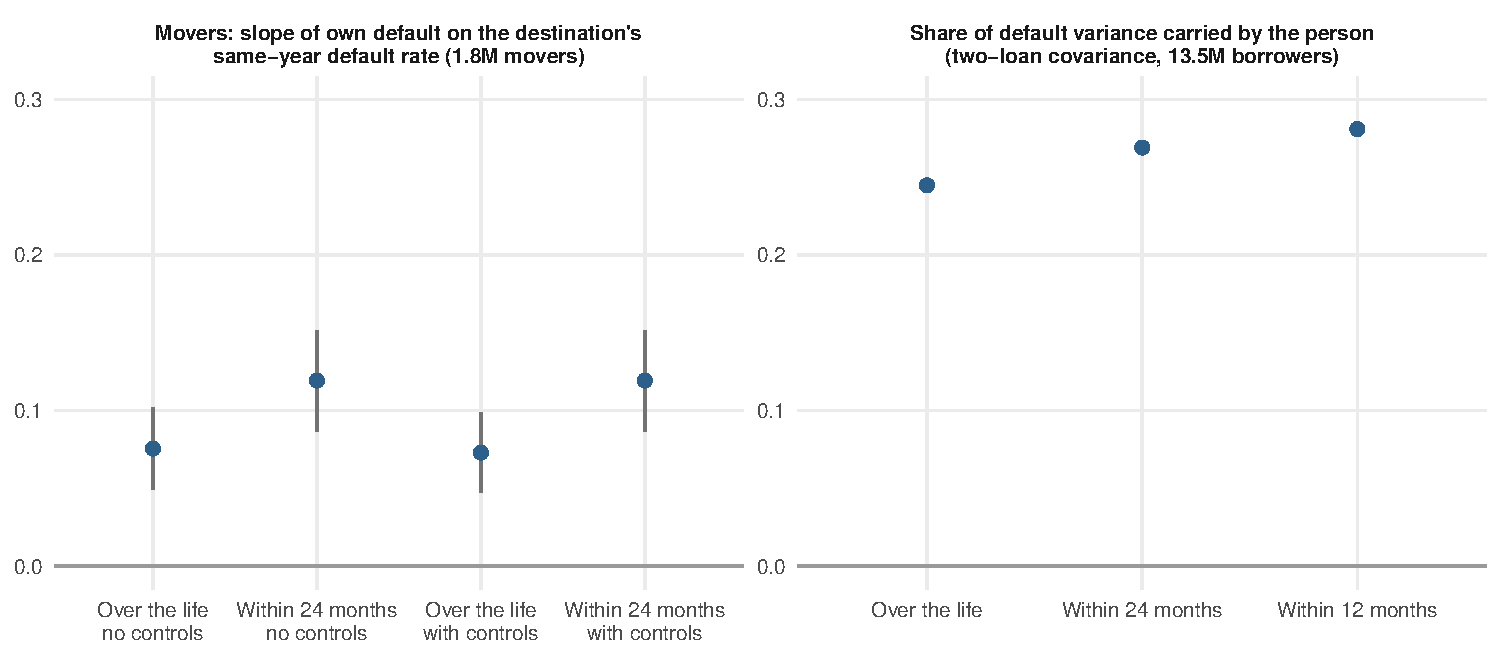
\includegraphics[width=0.48\textwidth,height=0.5\textheight,keepaspectratio]{figures/fig_place.pdf}\hfill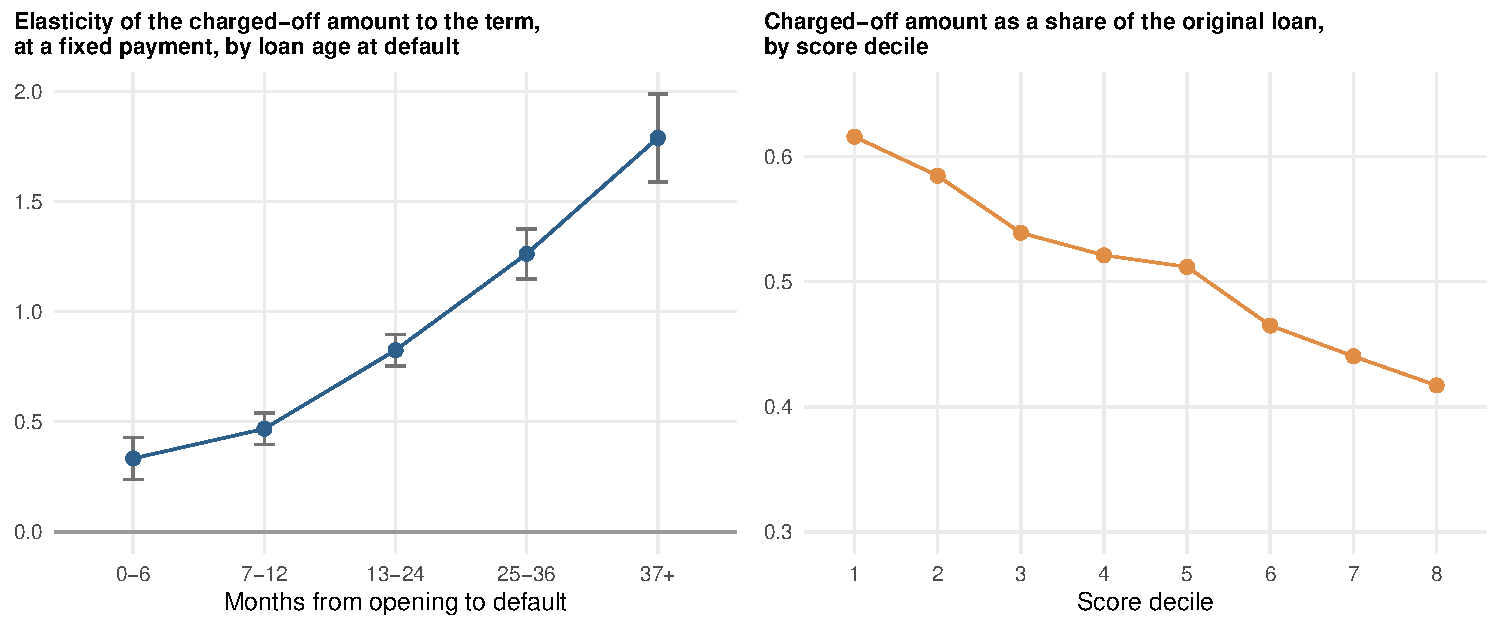
\includegraphics[width=0.48\textwidth,height=0.5\textheight,keepaspectratio]{figures/fig_chargeoff.pdf}
\begin{itemize}\small\m{A quarter of the variance of default is the person, and the place is 7 to 12 percent. Charge-off amounts scale one-for-one with the payment and increasingly with the term as the balance amortizes.}\end{itemize}\backto
\end{frame}

\begin{frame}{Power-preserving splits}
\centering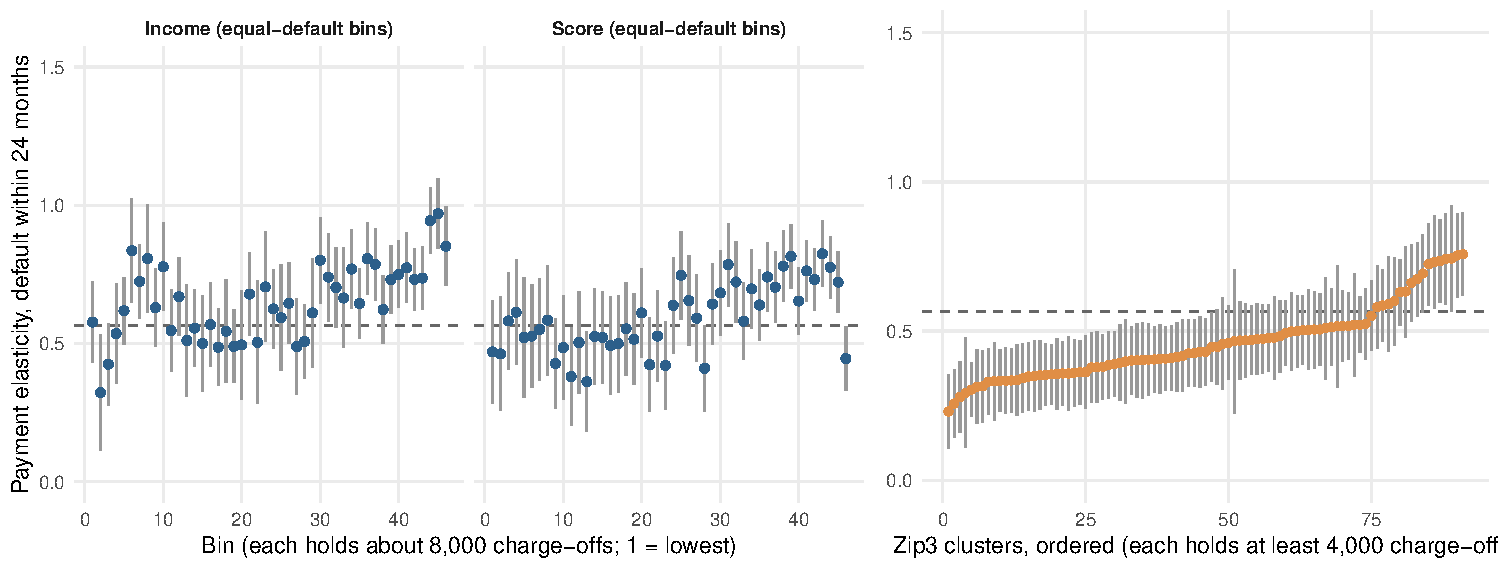
\includegraphics[width=\textwidth,height=0.6\textheight,keepaspectratio]{figures/fig_exposure_geo.pdf}\backto
\end{frame}

\begin{frame}[label=bk-runoff]{The model's run-off across discount rates}
\begin{itemize}\small
\m{Calibrated to the sample's default rate with anticipated exits at the measured hazard, the run-off ratio is $0.77$ to $0.82$ at every rate from $0$ to $1.2$, and the data's $0.75$ (charge-off) and $0.67$ (90-day) lie within.}
\m{The first-order formula, applied to the model's own simulations at true rates of $0.03$ to $0.10$, returns rates near $3$, because it includes survival and $\lambda$ but not the option.}
\m{At twice the taste-shock scale the elasticity level stays near five and the shape is unchanged. The model with i.i.d.\ income cannot reach the data's level at the data's default rate, and the level is where model and data are to be reconciled.}
\end{itemize}\backto
\end{frame}

\begin{frame}{Identification strategies tried}
\begin{itemize}\small
\m{Reading the rate off the default margins. The two separate logits, the closed form $x/(e^x-1)$, fixed-window outcomes.}
\m{Instruments for the term margin. Macro rates, size menus, leave-out lender menus, the 72-month menu discontinuity, the difference estimator under equi-confounding, within-borrower effects, selection on observables.}
\m{Separating channels. Deficiency rules, full model inversion, the first-order formula, contract-length bins, charge-off amounts.}
\m{Timing inside the bureau. Deferrals and balloons, pandemic forbearance, movers.}
\m{A rate by place. Net of collection law the state ratios stay outside the range (28 of 50); in place-by-score-tercile cells with the place fixed at the borrower's first loan, 34 of 96 state cells lie inside, the Northeast and Florida with rates and the South with bounds. Within tercile the term response is highest where the vote is Republican and lowest on the West Coast, beyond the bound in both directions.}
\m{The appendix records each with the object it would have identified and why it fell short, and the timing designs built and queued.}
\end{itemize}\backto
\end{frame}
\end{document}
